
\documentclass{article}
\usepackage{float}
\usepackage{tabularx}
\usepackage[utf8]{inputenc}
\pagenumbering{arabic}
\usepackage{graphicx}
\usepackage{amsmath}
\usepackage{caption}
\usepackage{authblk}
\usepackage{subcaption}
\begin{document}

\title{Connecting genes with evolutionary knowledge  using semantic similarity and ancestral profiles of variation}
\author[1]{Prashanti Manda\thanks{manda.prashanti@gmail.com}}
\author[1]{James P. Balhoff\thanks{balhoff@unc.edu}}
\author[2]{Hilmar Lapp\thanks{hilmar.lapp@duke.edu}}
\author[3]{Paula Mabee\thanks{paula.mabee@usd.edu}}
\author[1]{Todd J. Vision\thanks{tjv@bio.unc.edu}}
\affil[1]{Department of Biology, University of North Carolina, Chapel Hill}
\affil[2]{Center for Genomic and Computational Biology,Duke University}
\affil[3]{Department of Biology, University of South Dakota}


\renewcommand\Authands{ and }


\date{\today}
\maketitle
\begin{abstract}
Ontologies, and semantic databases annotated using ontologies, are increasing in number, size, and complexity, particularly in the life sciences. This growth necessitates the development of scalable approaches for reasoning over semantic databases in which large stores of data are annotated using multiple, large ontologies and also the development of statistical approaches for evaluating the large numbers of approximate matches that will results from a semantic similarity search. Here, we address these challenges in the context of the Phenoscape Knowledgebase, a semantic database containing over [320589 + no of evolutionary phenotypes (Jim?)] phenotypes from model vertebrate genetic studies and the evolutionary biology literature, annotated using terms from multiple, large ontologies. We describe three methods that allow the Phenoscape Knowledgebase to report biologically meaningful semantic similarities between phenotypes from these two different sources. First, we infer evolutionary phenotype variation using an ancestral reconstruction algorithm to reduce the search space and increase the biological relevance of the results. Second, we introduce techniques to efficiently reason over annotations that include multiple, large ontologies. Lastly, we present a statistical framework to rank semantic similarity results.
% Our results demonstrate that...  [fill in]

\end{abstract}

% Do you have a citation for method used? (original published source, not website!)

% This deserves more explanation, as it central to the methods.  Clarify what is already done by Uberon versus what is new to this work.
%"Ontology  bridges  and  equivalences  built  and maintained by the Uberon community are added to ensure inter-operability between these disparate ontologies.  Then, additional classes called subsumer classes representing combinations between Entity and attribute level quality classes are added to enable reasoning over EQ annotations.  As described above, these additional classes are added so that EQ annotations  can  be  subsumed  by  these  classes  or  so  that these  classes  establish  a  reasoning  chain  leading  to  other subsumers in the ontology".


%7. Table of top hits, some evidence for plausibility of top hits?

%%%%%%
% Comments from Hilmar (the chat function seems to be crude)
%
% Assuming that the comments above are Todd's, mine would be very similar:
%
% 1. To be a research paper, this needs to rise above a more detailed method description, and focus on what the new contributions are, what objective they are trying to accomplish, and provide illustration, evidence, and discussion of how well those objectives are being accomplished at this point.
%
% 2. I think the main contributions, and thus the focus topics for the paper are (i) using the Fitch parsimony algorithm for assigning evolutionary phenotype variation profiles, and (ii) calculating expect values through a multivariate linear regression followed by calculating probabilities for (studentized) residuals. 
%
% 3. This has to imply that (i) and (ii) can't just be sections in the methods section. The challenges that motivated us to devise these methods have to be in, and take center in the Introduction. There has be evidence presented that the devised methods are justified and work as intended. For the Fitch parsimony method, I think this has to include some idea of how the profile sizes co-vary with depth in the tree (which would need to be rank, presumably), and how this compares to "normal" character state matrices (is it similar? very different?). For the Expect score calculation, I think some example figure(s) of such a regression and with the residuals has to be presented. Also, evidence (ideally a figure) of how similarity score and expect score co-vary.

% 4. Various other comments:
%   (a) Frequency axes in figure should be logarithmically scaled,
%   (b) The description of Fitch algorithm at present is very confusing.
%   (c) The equivalences in Figure 2 are probably (and hopefully) not what you make them out to be. I think what you mean to illustrate is equivalence to the intersection of the Uberon and PATO terms.
%   (d) Most of the results are presented as de-facto. That's fine if the focus is on the biological discovery and the methods aren't flawed in some obvious manner. But for this paper, there needs to be evidence each time on what the results _mean_ for the algorithmic merits, limits, and generality of the method.

\section{Introduction} 

By allowing shared and computationally amenable representation of scientific knowledge, ontologies enable interoperability between data from heterogeneous sources \cite{uschold1996ontologies, blake2004bio} and allow for inference of new information where data is sparse or missing \cite{dececchi2015toward,maetschke2012gene}. More relevantly, this approach of knowledge representation enables semantic similarity - the matching of objects based on partial similarity of their ontology-driven conceptual representations. This capability has become paramount for many applications, particularly, in the life sciences where data in semantic databases are represented using logical statements composed of individual ontology terms. The growth of these semantic databases has spurred an increased interest in the application of semantic similarity measures to power database queries \cite{pesquita2009semantic, harispe2014semantic}. Many of the early applications involve estimating similarity between gene products and annotations based on the Gene Ontology (GO) \cite{gene2015gene}, such as \cite{mistry2008gene, couto2007measuring, couto2003implementation,yu2010gosemsim, du2009g, wu2013improving}.  More recently, a number of approaches to prioritize candidate genes for human diseases based on semantic similarity of phenotypes have been introduced \cite{oellrich2012improving, washington2009linking, chen2007improved}. 

The increased adoption of semantic databases, and semantic similarity search, in the life sciences introduces several scaling challenges. First, ontologies themselves tend to grow in size over time \cite{yang2006evaluation}. For instance, the GO has grown from about 18,000 classes in 2004 to 41,126 classes at the time of writing (May 15, 2015). Second, repositories of annotation data are growing. The GO annotation database \cite{?} has grown from 48 annotations in 1999 to more than 3.7 million at the time of writing. Individual annotations may use a growing number of ontologies. For example, phenotype annotations in animal models such as zebrafish typically include terms from Uberon \cite{haendel2014unification}, GO, the Phenotypic Trait Ontology (PATO) \cite{gkoutos2004using}, and the Biological Spatial Ontology (BSPO) \cite{dahdul2014nose}. When individual annotations use multiple, large ontologies, even relatively simple reasoning tasks can become computationally prohibitive. For example, the phenotype annotation describing absence (PATO:0000462) of the "alary process of premaxilla" (UBERON:3000003) uses classes from Uberon and PATO necessitating reasoning over more than 34 million combinations of Uberon and PATO classes. 

Here, we address these scalability issues in implementing semantic similarity search for the Phenoscape Knowledgebase \cite{manda2015using}, a semantic database of phenotypes described in more detail in section \ref{kb}. The contributions of this study are threefold. First, we take advantage of the evolutionary relationships inherent in the structure of the problem to infer new data, reduce the search space, and increase the biological relevance of the search results.  Second, we describe methods for reasoning over multiple, large ontologies through the collective use of class equivalences, special subsumer classes that combine classes from multiple ontologies, and by reduction of the granularity of phenotype annotations. Third, we introduce the use of extreme value statistics for ranking and reporting results from a semantic similarity search, including a consideration of how differences in ontology usage between annotation sources may affect the results.

%In addition, the structure and semantics of ontologies allow for inference of new information from annotation data, which is particularly useful in domains where annotated data is sparse or missing \cite{dececchi2015toward,maetschke2012gene}


\subsection{Phenoscape}
\label{kb}

The Phenoscape project uses ontologies to connect phenotypes reported in evolutionary literature with gene phenotypes that have been described for model organisms \cite{dahdul2010evolutionary,mabee2012500}. Phenotypes are annotated using the Entity Quality (EQ) annotation format (\cite{mungall2010integrating}). The Entity ({\it e.g.} `anal fin') is drawn from one ontology, such as the animal anatomy ontology Uberon \cite{haendel2014unification}, and the Quality ({\it e.g.} `elongated') that describes how the Entity is affected is drawn from a trait ontology, such as PATO \textbf{cite} \cite{mungall2010integrating}. More complex EQ annotations might contain an optional related entity (RE) and might post-compose multiple entities joined by relations from the Relations ontology (RO) and/or BSPO ({\it e.g.} 'sensory pore' (Uberon) 'dorsal\_to' (BSPO) 'orbital region' (Uberon)). The set of annotations, EQ or otherwise, used to describe an object is referred to as the object's profile. For example, the set of annotations describing a mutated gene's phenotypes is called the gene's phenotypic profile. 

The Phenoscape Knowledgebase (KB) currently contains [ ] Jim  annotations that correspond to 19,547 evolutionary character states in 4,895 vertebrate taxa, 3,935 of which are terminal. Evolutionary phenotypes largely involve the skeleton, and Phenoscape has particularly targeted the fin and limb appendages. These are combined with phenotypes for 3050 human, 7758 mouse, 5109 zebrafish, and 12 \textit{Xenopus} genes from the Human Phenotype Ontology \cite{kohler2013human}, Mouse Genome Informatics, \cite{eppig2015mouse}, Zebrafish Information Network \cite{bradford2011zfin}, and Xenbase \cite{karpinka2015xenbase}, respectively.  



%%% Brief three things. 


\subsection{Inference of evolutionary variation among taxa}
We present an inference method that propagates directly annotated phenotypes from thousands of terminal species in the taxonomic tree to higher taxonomic levels to infer evolutionary variation at those levels. The gamut of phenotypic diversity as a result of millions of years of evolution is typically described in phylogenetic studies using characters consisting of one or more states that vary along some aspect of the described character. For example, the character "basihyal bone shape" might have states "triangular" and "Y-shaped" in different species. Closely related species share character states while distantly related species have greater variability in their character states. Due to these properties, the study of variability in character states at different levels in the taxonomic tree can lead to an understanding of the phenotypic changes that might have occurred at different points of evolutionary history. However, such a study of evolutionary variation is currently not possible without computational inference methods due to missing or sparse phenotype annotations at higher taxonomic levels.  

Along with inferring missing phenotype data, our method reduces the search space of taxa to the subset of locations on the taxonomic tree where phenotypes vary among the daughter lineages, rather than the larger number of taxa with phenotypes reported in the literature. Thus, we apply domain knowledge to infer phenotype data and reduce the semantic similarity search space without sacrificing, or even increasing, the relevance of the results.

\subsection{Semantic search of evolutionarily variable taxa to a query model organism gene}

Here, we connect model organism gene phenotypes to evolutionarily varying taxon phenotypes through semantic similarity of their phenotypes. Parallel to the study of evolutionary phenotypes and phenotypic diversity, model organism communities have studied phenotypes resulting from genetic perturbations of specific genes. Connecting evolutionary variation to knowledge from developmental genetics can expand our understanding of both evolutionary variation and genetics. 

Semantic similarity is the process of assessing the degree of partial relatedness between entities such as genes, taxa etc. based on their annotations \cite{pesquita2009semantic}. There are several semantic similarity measures (see Pesquita et al. \cite{pesquita2009semantic}), some that primarily use the ontology structure while others also use statistics computed from annotations such as Information Content (IC). IC captures the rarity of an annotation in an annotation database with the assumption that rarely annotated concepts provide more information as compared to those that are frequently annotated. 


Since the IC of an annotation is dependent on the reference database, an annotation's IC might vary in different domains and different databases. This is particularly relevant to applications such as ours that conduct semantic searches over data from different domains (model organism communities, evolutionary biology). For example, a particular phenotype might not be well studied or annotated from an evolutionary perspective thereby making it rare and informative among taxa. However, the same phenotype might be extensively studied and annotated to model organism genes making it uninformative among genes. These differences in annotation cause disparities in annotation IC among genes vs. taxa. From the perspective of matching genes to taxa with evolutionary variation, it is a matter of concern when annotations contributing to semantic similarity are substantially more informative among taxa as compared to genes. We define a metric called IC Disparity score $D$ to quantify difference in annotation IC among genes vs. taxa. 

A common theme among most semantic similarity metrics is the inference of annotation subsumers/ancestors from the ontology typically accomplished by ontology reasoners such as Elk \cite{kazakov2014incredible}. However, for our application, subsumer inference is challenging due to the use of disparate annotation formats (pre- vs post-composed) and multiple ontologies to represent phenotypes. 

\subsection{Pre-composed versus post-composed phenotype annotations}
The mouse and human annotation sources use pre-composed phenotype ontologies, meaning that the affected anatomical entity and the effect (quality) are expressed in the same ontology concept. For example, the concept "calcified muscle" from the Mammalian Phenotype ontology \cite{smith2012mammalian} combines the entity ("muscle") and the quality "calcified". Mouse gene phenotypes are described using mammalian phenotype ontology \cite{smith2012mammalian} while human gene phenotypes use the human phenotype ontology (HPO) \cite{kohler2013human}. 

In contrast, evolutionary phenotypes are primarily represented using the post-composed Entity-Quality (EQ) format \cite{mungall2010integrating}. The use of post-composed EQ annotations is challenging for subsumption reasoning to compute semantic similarity since the lack of a unified pre-composed ontology prevents the inference of subsumers for EQ annotations.  One way to address the lack of a pre-composed EQ ontology is to create a comprehensive ontology with EQ classes from the cartesian product between the sets of Entity classes from Uberon and Quality classes from PATO (see fig. 3 in \cite{washington2009linking}). However, this combinatorial EQ ontology is prohibitively large for even the fastest reasoners.  

The ontology space may be reduced in several ways, one of which is by reducing the annotation granularity on one or more of the ontologies. In the case of EQ annotations, the granularity of PATO can be restricted by using only a set of high level classes called attributes, analogous to GO slims \cite{gene2004gene}. At the time of writing (April 30, 2015), Uberon contains 14,032 classes, the full PATO contains 2457 classes, and the attribute level PATO contains 15 classes. Reasoning over attribute PATO classes instead of the full PATO would reduce the combinatorial EQ ontology space from over 34 million classes to about 210,000 which is still substantially large. The computational challenges of reasoning over this large ontology are significant and require scalable solutions that enable reasoning over EQ annotations.  

Second, disparate multiple phenotype ontologies can be connected using class equivalences. For example, a set of class equivalences between MP, Uberon, and PATO describe MP classes as intersections of Uberon and PATO classes (fig. \ref{equivalence}). These equivalences partly establish the ontology structure that links pre-composed phenotype annotations to post-composed EQ annotations.  


\begin{figure}
\centering
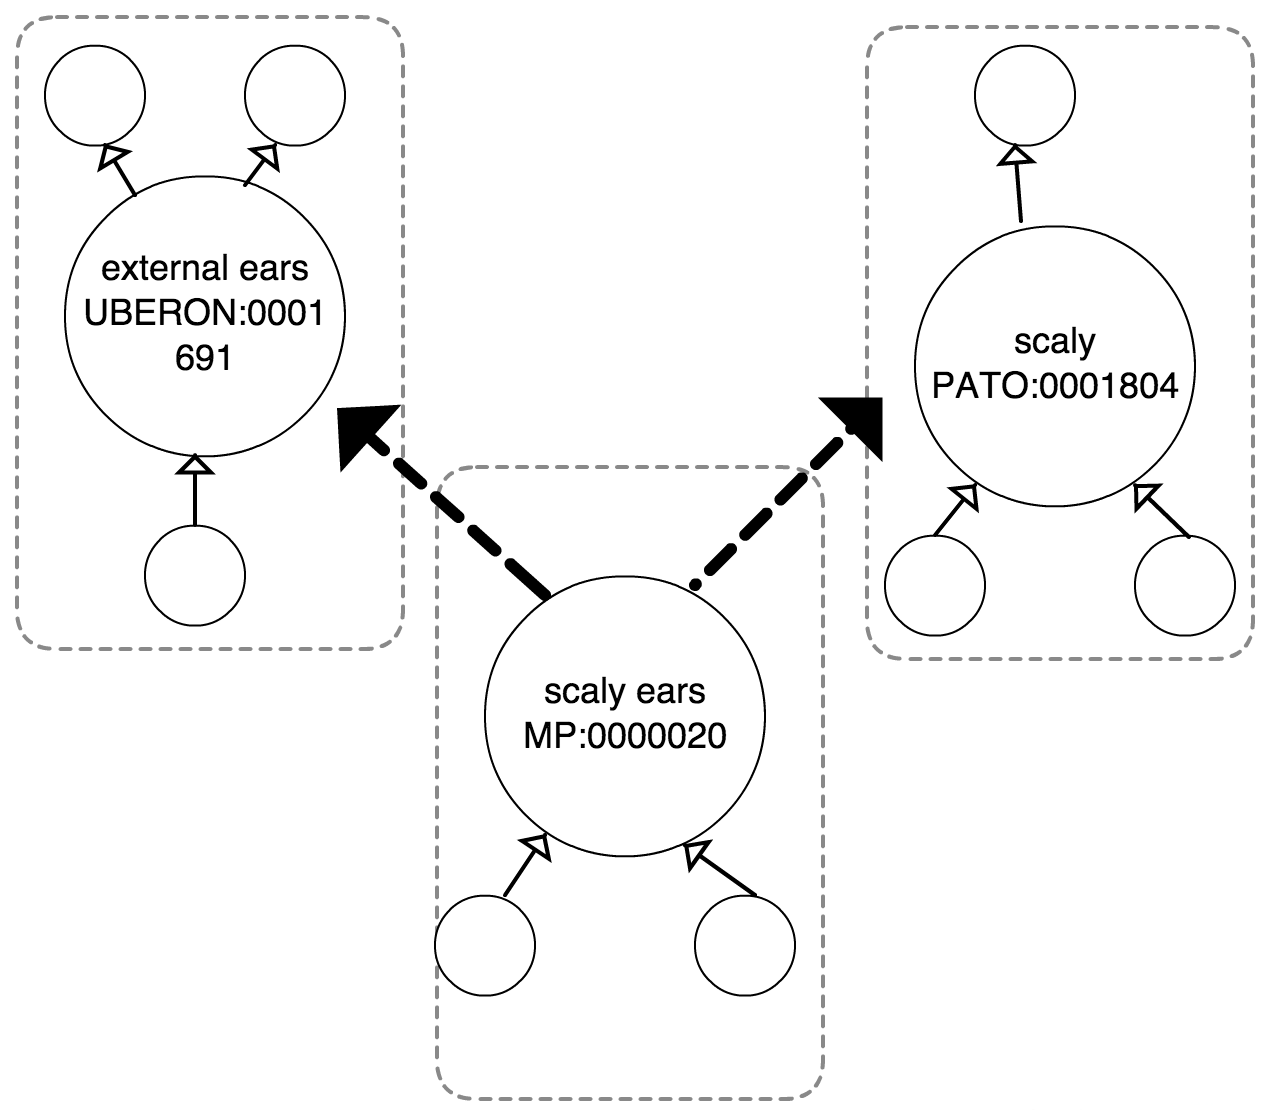
\includegraphics[width=1\textwidth]{Equivalence.png}
\caption{\label{equivalence} Example of an equivalence axiom relating the Mammalian phenotype (MP) class \textit{"scaly ears"} to the Uberon class \textit{"external ear"} and the Quality (PATO) class \textit{"scaly"} thus establishing connectivity between MP, Uberon, and PATO ontologies and between MP and EQ annotations.}
\end{figure}



\subsection{A statistical framework for estimating significance of ontological semantic searches}

As the size of a semantic database grows, it becomes increasingly important to have a statistical framework for evaluating the results from a semantic similarity search. Many approximate matches will be returned, and so the user wishes to understand both the relative strength of the matches and to know how strong a match needs to be in order to merit interest. The size of the database will affect how likely we are to see the best match achieve a given score and, depending on the measure used, the score may also be influenced by other factors that vary among search objects (such as the number of annotations being compared). Bioinformaticians are well acquainted with the statistical methods that have been developed to evaluate sequence similarity scores from database searches of gene or protein sequences \cite{pearson1998empirical, altschul1997gapped}.To our knowledge, similar ideas have yet to be applied to semantic similarity search. Most current semantic similarity applications rank search results based on similarity scores directly \cite{washington2009linking, harispe2014semantic, smedley2013phenodigm}, but see Bauer and collegues \cite{bauer2012bayesian}, who model the probability of a match between a disease and complex phenotype using Bayesian networks.

\section{Methods}

\subsection{Inference of evolutionary variation among taxa}
Profiles of evolutionary variation are inferred for each node in the taxonomic tree from the original character state data using a maximum parsimony ancestral state reconstruction algorithm modified from \cite{fitch1971toward}. The inputs to the algorithm are the taxonomic tree in the form of the VTO, character states associated with nodes in the tree, and mappings between character states to one or more EQ annotations.

The reconstruction algorithm attempts to infer phenotypic and evolutionary profiles for each non-terminal node in the taxonomic tree. A node's phenotypic profile is either the set of character states directly annotated to the node or the set of inferred character states based on its children's phenotypic profile. A node's evolutionary profile is the set of character states inferred to be variable among its children's phenotypic profiles.   

For each character, the reconstruction algorithm conducts a post-order traversal of the tree proceeding from the tips toward the root of the tree, inferring the set of possible character states (phenotypic profile) for each internal node based on the observed character states of the node's children. During this process, phenotypic profiles of parent nodes are built by adding the intersection of their children's states for every observed character. Children with missing data are excluded from this intersection calculation. If a parent node is directly annotated to a state for a given character, the state is added to the computed intersection. 

In cases when there is no intersection in the states of a character among the children of a parent node, we deem the character to be evolutionarily varying at the parent node level. These varying states (union of the children's states for the character) are added to the evolutionary profile of the parent node indicating that there is variation among the members of this clade with regard to these character states (Fig \ref{fitch}). This process continues recursively back to the root of the tree. At the end of the algorithm execution, character states collected in the evolutionary profiles for each taxon are replaced by their corresponding EQ annotations. 

\begin{figure}
\centering
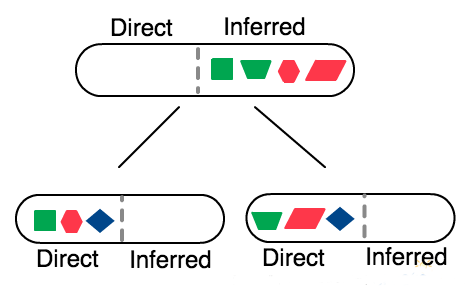
\includegraphics[width=1\textwidth]{ACM-Fitch.png}
\caption{\label{fitch} Inference of evolutionary profiles for nodes on the taxonomic tree. Colors represent characters and shapes represent states of the character. In this example, there are three characters (green, red, and blue) and 5 states associated with them. Each node has a direct phenotype profile and an inferred evolutionary profile.}
\end{figure}

\subsection{Semantic Similarity}
The set of all EQ annotations representing variable character states for a taxon form its evolutionary profile (a.k.a taxon profile). Similarly, the set of all phenotype annotations to a model organism gene forms its gene phenotype profile. Semantic similarity between a gene profile and a taxon's evolutionary profile, called overall similarity ($S_O$), is defined as the median of the best individual semantic similarities ($S_A$) for every gene annotation to taxon evolutionary profile annotations. For a gene profile with $Y$ annotations, the median is computed from the $Y$ best matches between gene to taxon annotations. Semantic similarity between a pair of annotations ($A_i$,$A_j$) is quantified using the following metrics. 

\subsubsection{Semantic Similarity Metrics}
\paragraph{Information Content ($IC$)}
Semantic similarity between a pair of annotations using $IC$ is defined as the Information content ($IC$) of the most informative common ancestor (MICA) of the annotations. 

\begin{equation}
\label{sa}
S_A (A_i,A_j) = IC(\textrm{MICA} (A_i,A_j))
\end{equation}

The $IC$ of a node (such as the MICA) $N_i$ in an ontology is defined as the negative logarithm of the proportion of the dataset (genes, taxa, etc.) annotated to $N_i$ or any node subsumed by $N_i$ \cite{resnik1999semantic}. Since our application focuses on retrieving similar taxa for a query gene, we estimate information content of a node (or MICA) based on the proportion of taxon profiles it is annotated to. Let there be $T$ taxa in the search database. Define $f(N)$ as the number of taxa annotated directly to $N_i$ or to any node subsumed by $N_i$. 
Mathematically, the $IC$ of the node, $N_i$ is defined as:

\begin{equation}
\label{IC}
IC(N_i) = -\log(p(N_i)), \\
\end{equation}
where
\begin{align*}
& p(N_i) = \frac{f(N_i)} {T}
\end{align*}

The minimum $IC$ score, which the ontology root must always take, is zero. The highest possible $IC$ score is dependent on the number of taxa. $IC$ scores are normalized ($nIC$) by dividing it with the maximum score possible ($IC_{max}$) so that it ranges from 0 to 1.
\begin{equation}
\label{nIC}
nIC(N_i)=\frac{IC(N_i)}{IC_{max}} \\
\end{equation}
where
\begin{align*}
& IC_{max}=-\log(\frac{1}{T})
\end{align*}


A score called IC disparity ($D$) quantifies the difference in informativeness of a MICA among the taxon evolutionary profiles as compared to the MICA's IC if the calculation had been done using the proportion of annotations among the gene profiles.

\begin{equation}
\label{disparity}
D=IC_T(\textrm{MICA})-IC_G(\textrm{MICA}) 
\end{equation}
where 
\begin{align*}
& IC_T(\textrm{MICA}) \textrm{ is the IC of the MICA among evolutionary profiles,} \\
& IC_G(\textrm{MICA}) \textrm{is the IC of the MICA among gene profiles.} \\
\end{align*}

A warning is displayed for annotation comparisons when $D$ is above a selected threshold. A threshold of 0.25 was selected for $D$ by examining the distribution of disparity scores for all MICAs. 

\paragraph{Jaccard Similarity ($SimJ$)}

\subsection{Semantic similarity reasoning}
\label{reasoning}
In the absence of a pre-composed EQ ontology, we built a comprehensive ontology ($C$) to enable integrated subsumption reasoning over post-composed EQ evolutionary phenotype annotations and pre-composed gene phenotype annotations. 

First, all classes from Uberon, PATO, BSPO, MP, and HPO were added to an empty $C$. Second, equivalence axioms that connect MP and HPO classes to Uberon and PATO were added to $C$. These inter-ontology equivalences provided by the Uberon community describe MP and HPO classes as intersections of the corresponding Uberon and PATO class (Fig. \ref{equivalence}). The addition of these equivalences connects HPO and MP classes through Uberon and PATO. At this stage, $C$ contains all the classes necessary to reason over the pre-composed gene annotations. 

Second, EQ annotations from all evolutionary profiles in the KB were added to $C$. This step is not required for gene profiles because gene annotations are pre-composed classes which have already been added in the first step. Each EQ annotation is converted into an OWL expression of the form "\textit{has\_part} some (Q and (\textit{inheres\_in} some E and \textit{towards} some RE))" or just "\textit{has\_part} some (Q and \textit{inheres\_in} some E)" if there is no related entity. Then, a class equivalent to the OWL expression is added to $C$. 

Finally, special EQ subsumer classes that represent combinations of Uberon and PATO attribute classes were generated to enable reasoning over EQ annotations. We define the following two OWL expression templates to combine Uberon entity classes with PATO attribute classes. For every Uberon ($E$), PATO attribute class ($Q_A$) pair, two classes equivalent to the following OWL expressions were added to $C$.

\begin{enumerate}
\item $has\_part$ some ($Q_A$ and $phenotype\_of$ some $E$)
\item $has\_part$ some ($Q_A$ and $phenotype\_of$ some ($part\_of$ some $E$))
\end{enumerate}

In the above templates, \textit{'has\_part'}, \textit{'part\_of'}, and \textit{'phenotype\_of'} are ontology object properties. \textit{'has\_part'} and \textit{'part\_of'} properties are from RO. The \textit{'phenotype\_of'} property is defined in $C$ as a super property of the \textit{'inheres\_in'} and \textit{'towards'} relations.


The reasoner can now infer appropriate subsumers for EQ annotations from the added EQ subsumer classes. In the absence of the EQ subsumer classes, the reasoner infers incomplete subsumers for EQ annotations only on the PATO hierarchy (fig. \ref{reasoninga}). The addition of the EQ subsumer classes enables the reasoner to identify appropriate subsumers for EQ annotations using both PATO and Uberon hierarchies (fig. \ref{reasoningb}). 


%The \textit{'has\_part'} property is reflexive meaning that annotations of the form "Q and ", '\textit{has\_part} some Q' will be subsumed under these classes. The \textit{'phenotype\_of'} property is added to the composite ontology as a super property of the \textit{'inheres\_in'} and \textit{'towards'}, to subsume annotations with Entity components that match either usage. 

\begin{figure}
\begin{minipage}{.5\textwidth}
  \vspace*{\fill}
  \centering
  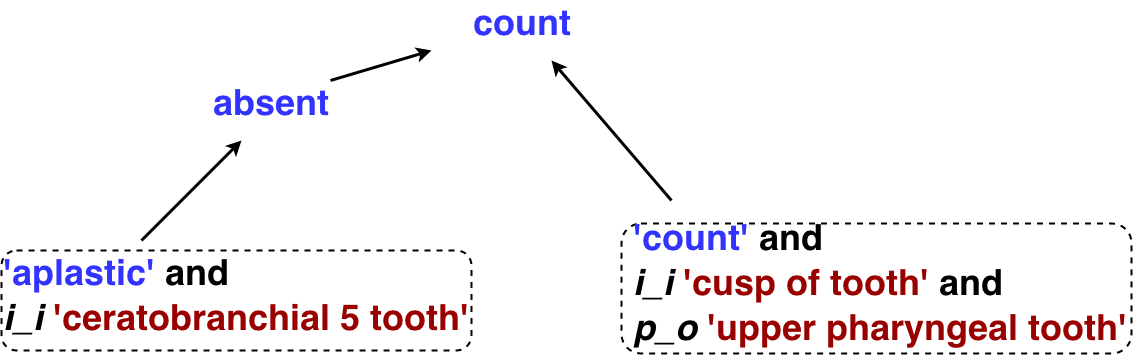
\includegraphics[scale=0.2]{reasoninga.png}
  \subcaption{The absence of appropriate EQ classes prevents proper subsumption reasoning. The reasoner identifies subsumers based only on the quality part of the annotation. The shared subsumer in this reasoning set up is 'count' thereby ignoring the entities entirely.}
  \label{reasoninga}\par\vfill
  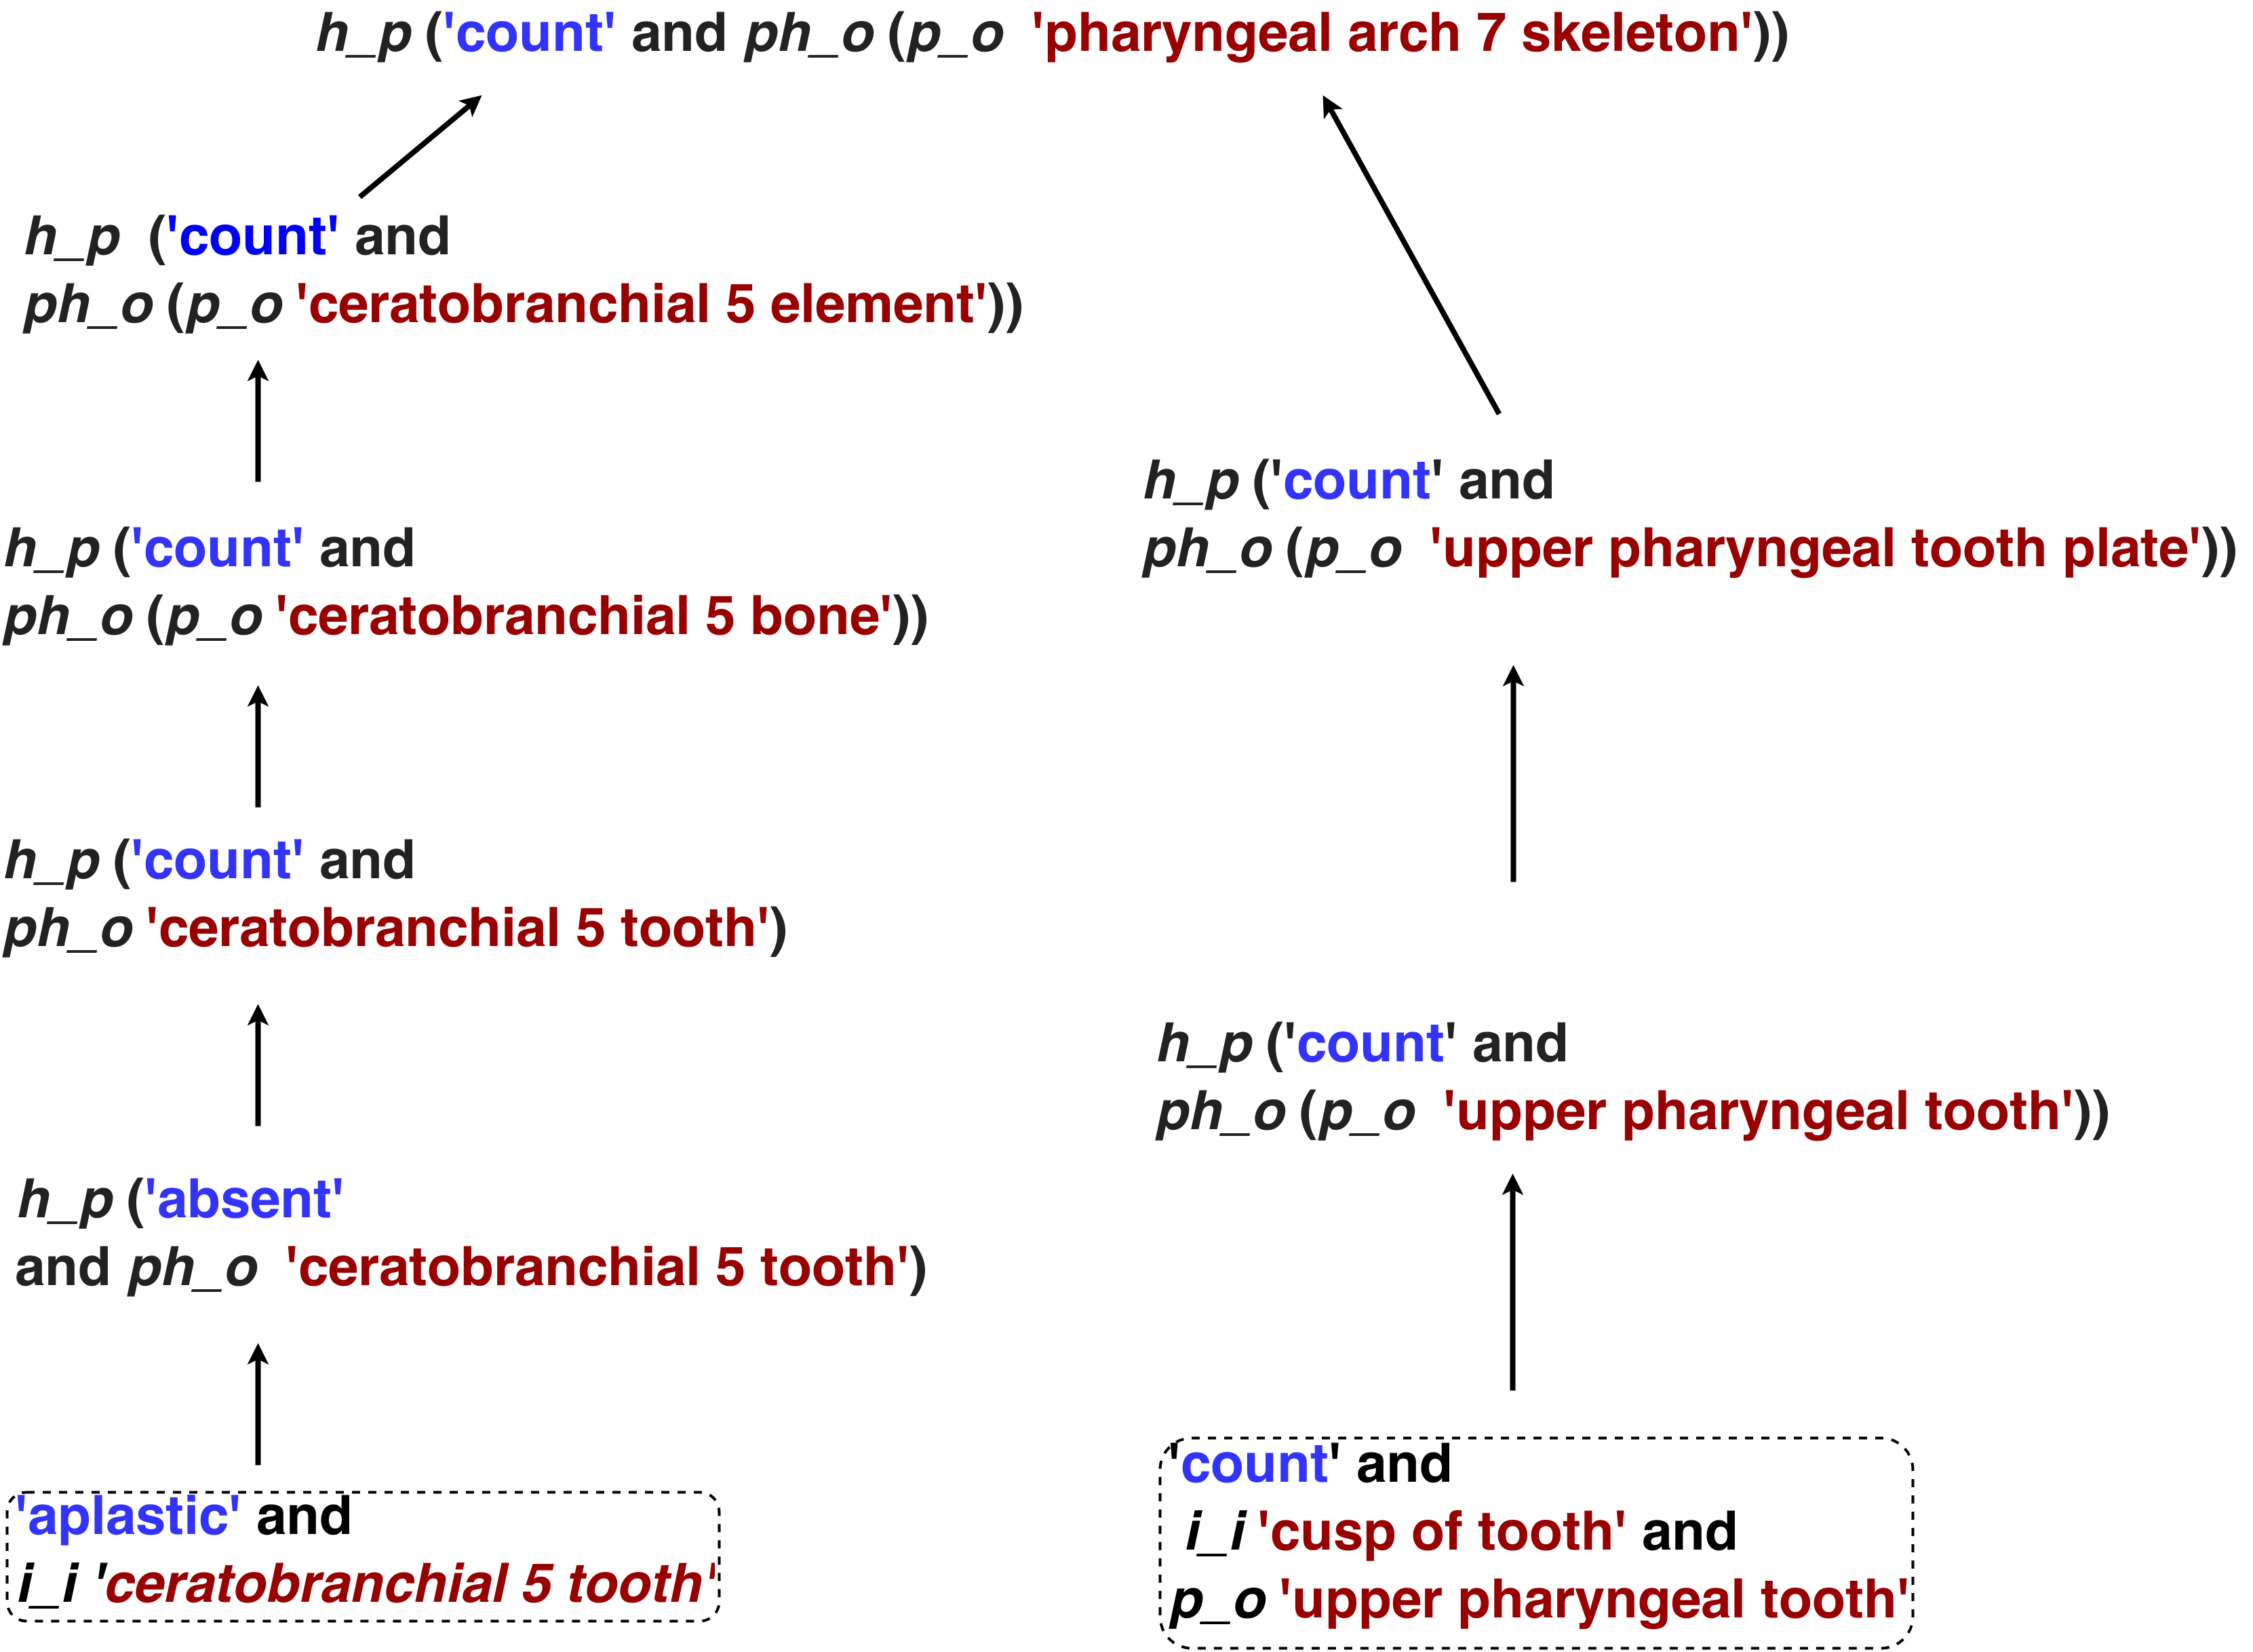
\includegraphics[scale=0.08]{reasoningb.png}
  \subcaption{Addition of EQ subsumer classes enables inference of subsumers that takes both entities and qualities into account. The shared subsumer in this reasoning paradigm is \textit{has\_phenotype} (count and \textit{phenotype\_of} (\textit{part\_of} 'pharyngeal arch 7 skeleton')).}
  \label{reasoningb}
\end{minipage}

\caption{Subsumption reasoning between a taxon evolutionary phenotype and gene phenotype (both in dashed boxes) before and after the addition of EQ subsumer classes.  Abbreviations used in figures: \textit{i\_i} - \textit{inheres\_in}, \textit{p\_o} - \textit{part\_of}, \textit{ph\_o} - \textit{phenotype\_of}, \textit{h\_p} - \textit{has\_part}}
\end{figure}


\subsection{Significance of a semantic similarity match}
Every semantic similarity match for a query is accompanied by an Expect ($E$) value which indicates the number of matches one expects to see for a given query with the same overall similarity or higher. To compute $E$ values, first, a multiple linear regression if performed using the Ordinary Least Squares method \cite{haggstrom1983logistic}.  The dependent variable is overall similarity and the independent variables are the log transformed genetic and evolutionary profile sizes. 

The regression model is

\begin{equation}
\label{regressionmodel}
S_O' = c + \alpha*X + \beta*Y \\
\end{equation}
where
\begin{align*}
&  i \textrm{is the intercept to be fit}\\
& X, Y \textrm{are the log of the evolutionary and genetic profile sizes, respectively} \\
& \alpha, \beta \textrm{are co-efficients to be fit}
\end{align*}

Raw residuals ($R_R$) are calculated as the difference between the actual ($S_O$) and predicted ($S_O'$) overall similarity.

\begin{equation}
\label{residual}
R_R=S_O - S_O' \\
\end{equation}

Studentized residuals ($R_S$) were calculated so that residuals from different data points could be directly compared (Equation \ref{studentize}).

% I modified the hat matrix notation -TJV 
%%% The symbol for the hat matrix is hii not h_ii. I changed it back. 

\begin{equation}
\label{studentize}
R_S = \frac{R_R}{\sigma \sqrt{1-h_{ii}}} \\
\end{equation}
where 
\begin{align*}
& \sigma \textrm{ is an estimate of the standard deviation of the residuals,} \\
& \textrm{hii is the diagonal of the hat matrix \cite{hoaglin1978hat}} \\
\end{align*}

% don't understand that explanation

The hat matrix hii is a map of the observed to predicted scores.

Next, the probability $p$ of obtaining a score greater than a given $S_O$ score is estimated from the extreme value distribution of the studentized residuals (Equation 4, \textbf{cite Pearson}).

\begin{equation}
\label{pvalue}
p=1-\exp \left( {-e^{\frac{-\pi R_S }{\sqrt{6} - \Gamma'(1)}}} \right) \\
\end{equation}
where 
\begin{align*}
& R_S \textrm{ is the Studentized residual,} \\
& \Gamma'(1) \textrm{ is the Gamma function evaluated at 1}
 \\
\end{align*}

The $E$ value is computed by multiplying $p$ (Equation \ref{expect}) by the size of the database, in this case the number of taxa with evolutionary profiles, $T=636$.

\begin{equation}
\label{expect}
E = pT = p636
\end{equation}


In our application of searching a database of taxon profiles for a query gene, it is a concern when overall similarity includes MICAs deemed informative for taxa but are known to be substantially less informative among genes (positive disparity scores).  %%We selected a threshold of 0.25 for positive disparity scores based on the disparity distribution to generate a IC warning when those MICAs appear in similarity comparisons. 

\subsection{Distinguishing semantic similarity from noise}
We conducted an experiment to demonstrate that our similarity metrics combined with expect score statistics have the power to identify  and distinguish real similarity distinguish it from background noise. 

To demonstrate this, we created a database of faux evolutionary profiles. For every evolutionary profile $P$, in the KB, a faux profile ($P'$) of the same size was created and added to the database. These faux profiles were populated by selecting annotations with uniform probability and without replacement from the pool of annotations constituting real evolutionary profiles. Annotation redundancies in real evolutionary profiles were preserved in the annotation pool. Randomly selected annotations were replaced into the annotation pool if they were already present in the faux profile to avoid annotation redundancy within a profile. 


Query profiles were selected iteratively from faux profiles with uniform probability and compared to all profiles in the faux database. Initially, the query profile matches itself in the database with a perfect similarity score. We hypothesize the expect score of this perfect match to be significantly lower than 1. 

Next, we incrementally dilute the perfect match between the query profile and the faux database by replacing one annotation in the query profile with a randomly selected annotation from the annotation pool that is not already present in the query profile. The query profile is compared to all profiles in the faux database after each annotation replacement. Each annotation replacement decays the similarity between the query profile and the initially matched profile in the faux database and results in decreasing similarity and increasing expect scores. The number of iterations a query profile undergoes is equal its number of annotations. The process ends when all annotations in the profile have been replaced with a randomly selected annotation. The last round of comparison between the query and faux profiles represents the baseline of similarity when profiles with no biological significance (noise) are compared to each other.  

\section{Results}
\subsection{Inference of evolutionary profiles}

%%% Update numbers in results
%% The Vertebrate Taxonomy Ontology was used as the structure for inference of evolutionary variation.  Version [X] Jim of the VTO contains 107,087 classes, or taxa \cite{midford2013vertebrate}. The Phenoscape KB contains phenotype annotations to 4,895 of these taxa, of which 3,935 (about 80\%) are terminals, or species. 6,815 unique characters with 17,940 character states contributed to inferred variation in 636 of the taxa upon application of the modified Fitch algorithm.  Each character state was translated into 1 to 8 EQ annotations, which resulted in a total of 23,691 unique EQ annotations. The profile sizes ranged from 2 to 2829 EQs with a median size of 31. Figure \ref{taxonsize}) shows that about 98\% of profile sizes are within 600.

%% \begin{figure}
%% \centering
%% 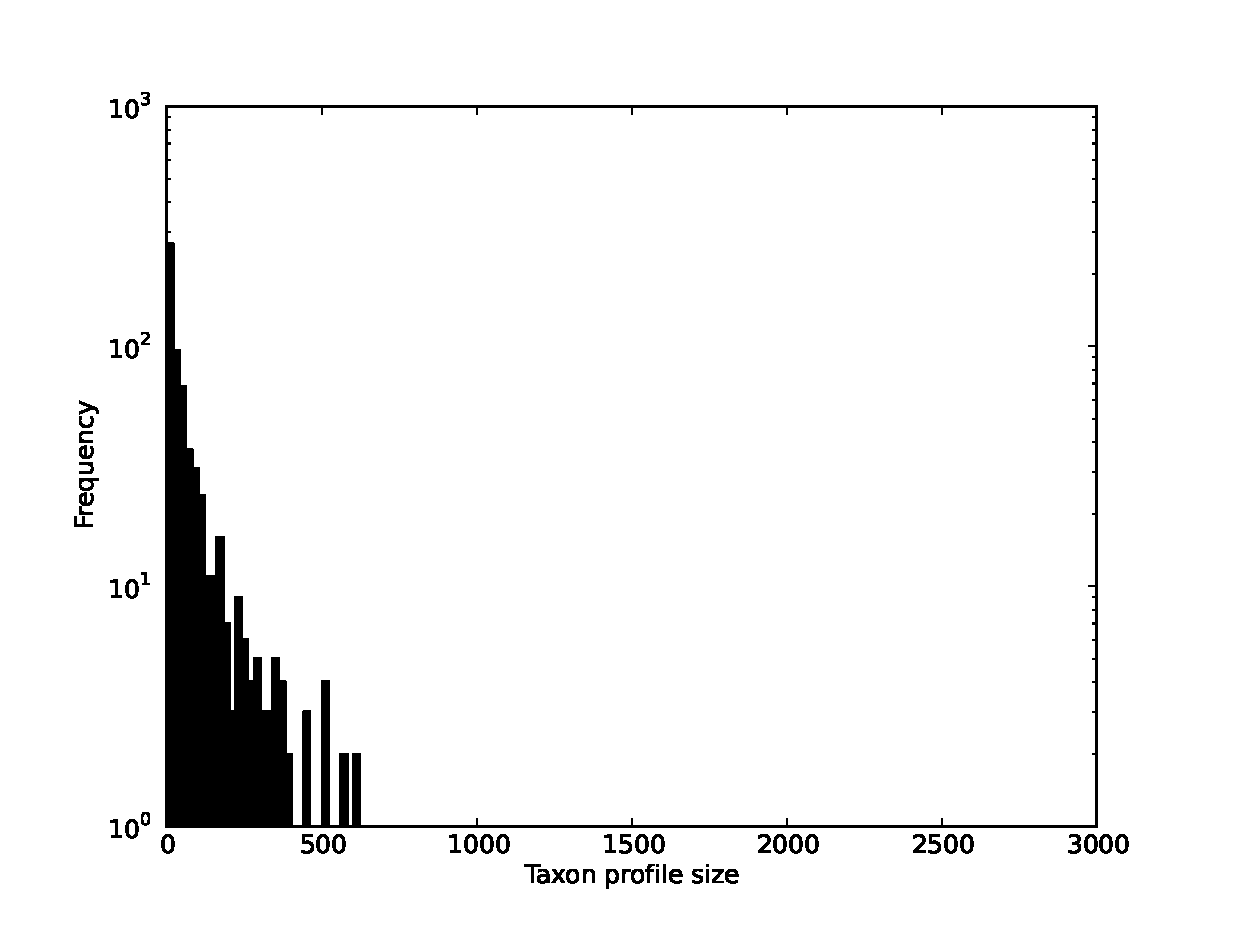
\includegraphics[width=1\textwidth]{TaxonSize-Histogram.eps}
%% \caption{\label{taxonsize} Distribution of taxon evolutionary profile sizes (number of EQ annotations). N = 636 evolutionary profiles.}
%% \end{figure}

\subsection{Semantic similarity between genetic and evolutionary profiles} 
%% The comprehensive ontology generated for semantic similarity reasoning contained approximately 751,830 classes, including 13,088 from Uberon, 2466 from PATO, 7153 from MP, 10,751 from HPO, and 534,533 subsumer and EQ annotation classes. 

%% A total of 10,130,844 semantic similarity comparisons were conducted between the 15,929 gene and 636 evolutionary profiles. overall semantic similarity scores for all gene–taxon comparisons ranged from 0 to 0.89 with a median score of 0.06.

\subsection{Computing expect values for semantic search results}
%% A linear regression model that that included gene profile sizes, taxon profile sizes as the independent variables and overall similarity as the dependent variable showed that approximately 32\% of overall similarity between a given gene and taxon profile could be explained by the sizes of the two profiles (Figs \ref{genesizes}, \ref{taxonsizes}).

%% \begin{figure}
%% \begin{minipage}{.5\textwidth}
%%   \vspace*{\fill}
%%   \centering
%%   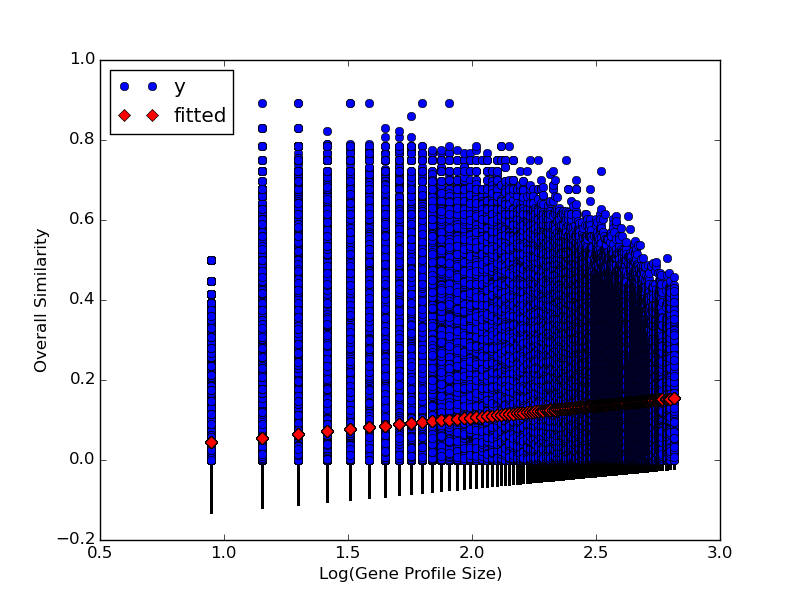
\includegraphics[scale=0.5]{Transformed_Regression_GeneSizes.png}
%%   \subcaption{Dependence of overall similarity between gene and taxon profiles on gene profile size.}
%   \label{genesizes}\par\vfill
%   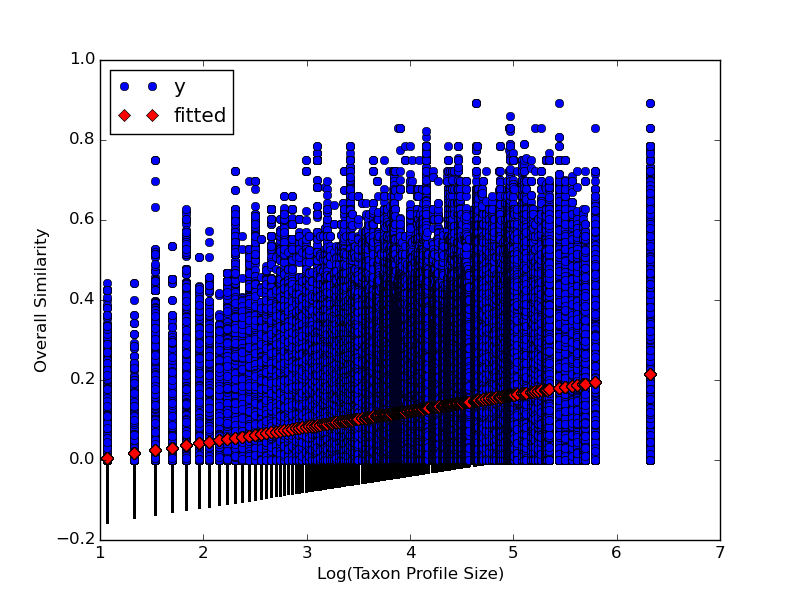
\includegraphics[scale=0.5]{Transformed_Regression_TaxonSizes.png}
%   \subcaption{Dependence of overall similarity between gene and taxon profiles on taxon profile size.}
%   \label{taxonsizes}
% \end{minipage}
% \label{regression}
% \caption{Linear regression with gene and evolutionary profile sizes as the independent variables and overall similarity as the dependent variable. $R^2=0.321$, 
% $S_O$ = (0.0593*$X$) + (0.0400 * $Y$) - 0.1352.
% }
% \end{figure}


%% Expect values of the best taxon matches for genes ranged from 4.42e-05 to 567.83. 0.08\% of all pairwise gene to taxon matches and 52.43\% of the best taxon matches had expect scores less than 1. Although the transformed linear regression substantially reduced the bias of overall similarity due to profile sizes, it was unable to remove all bias \ref{genesizes},\ref{taxonsizes}. 0.0003\% of profiles with log size in the range [1,2] have expect scores less than 1 in the set of best taxon matches as compared to 0.0005\% of profiles with log size [7-8]. This indicates that taxon profiles in the highest size range are 1.62 times more likely to have significant expect scores as compared to the smallest size range. 


%% The cumulative distribution of significant similarity results shows a curve rather than the expected extreme value distribution straight line indicating biologically significant results stronger than expected by chance (Fig. \ref{expectcumulative}). 

% \begin{figure}
% \centering
% 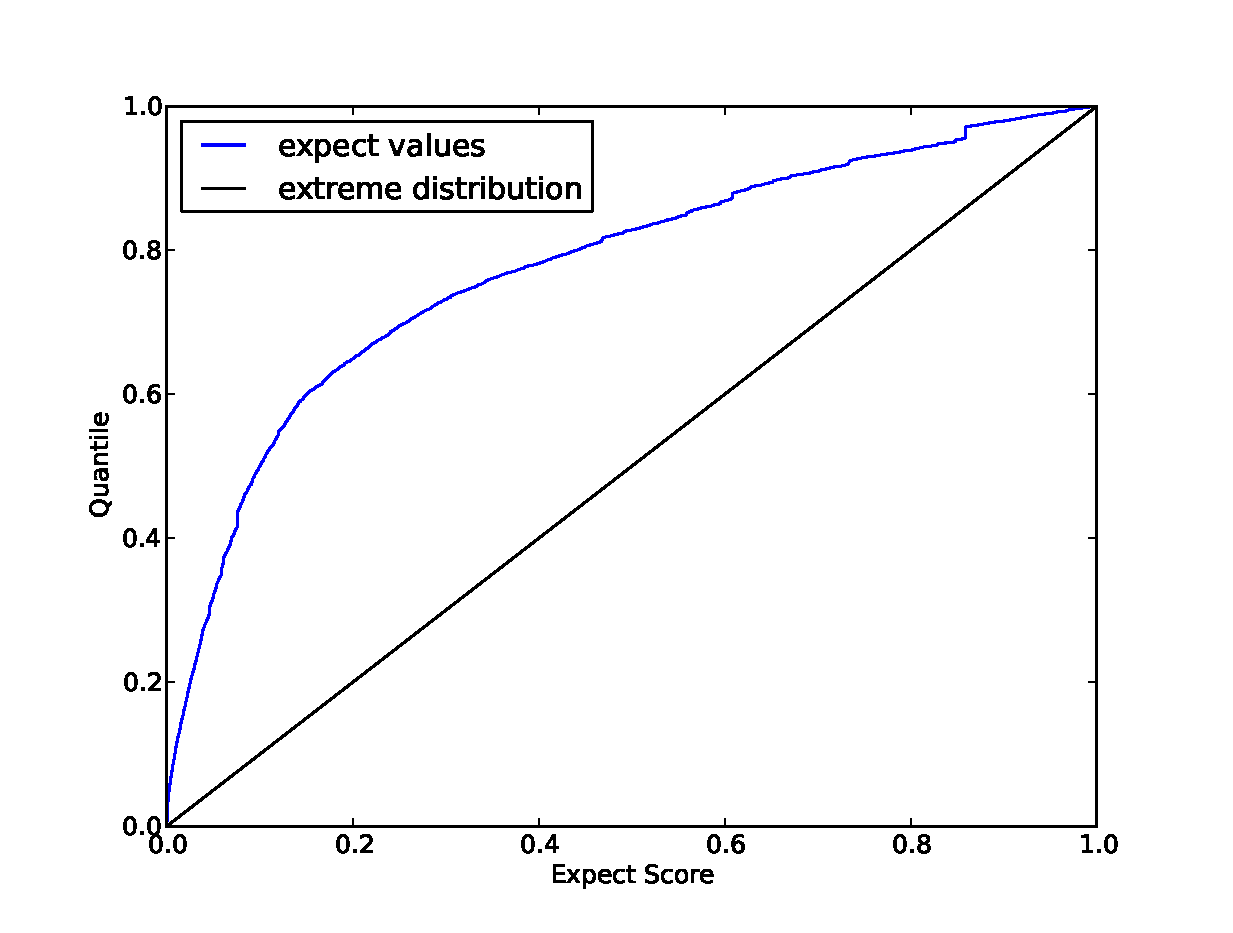
\includegraphics[width=1\textwidth]{Expect-Cumulative.eps}
% \caption{\label{expectcumulative}Q-Q plot of the cumulative distribution of significant expect values for the best taxon match for every gene vs expected quantiles.}
% \end{figure}

%\begin{figure}
%\centering
%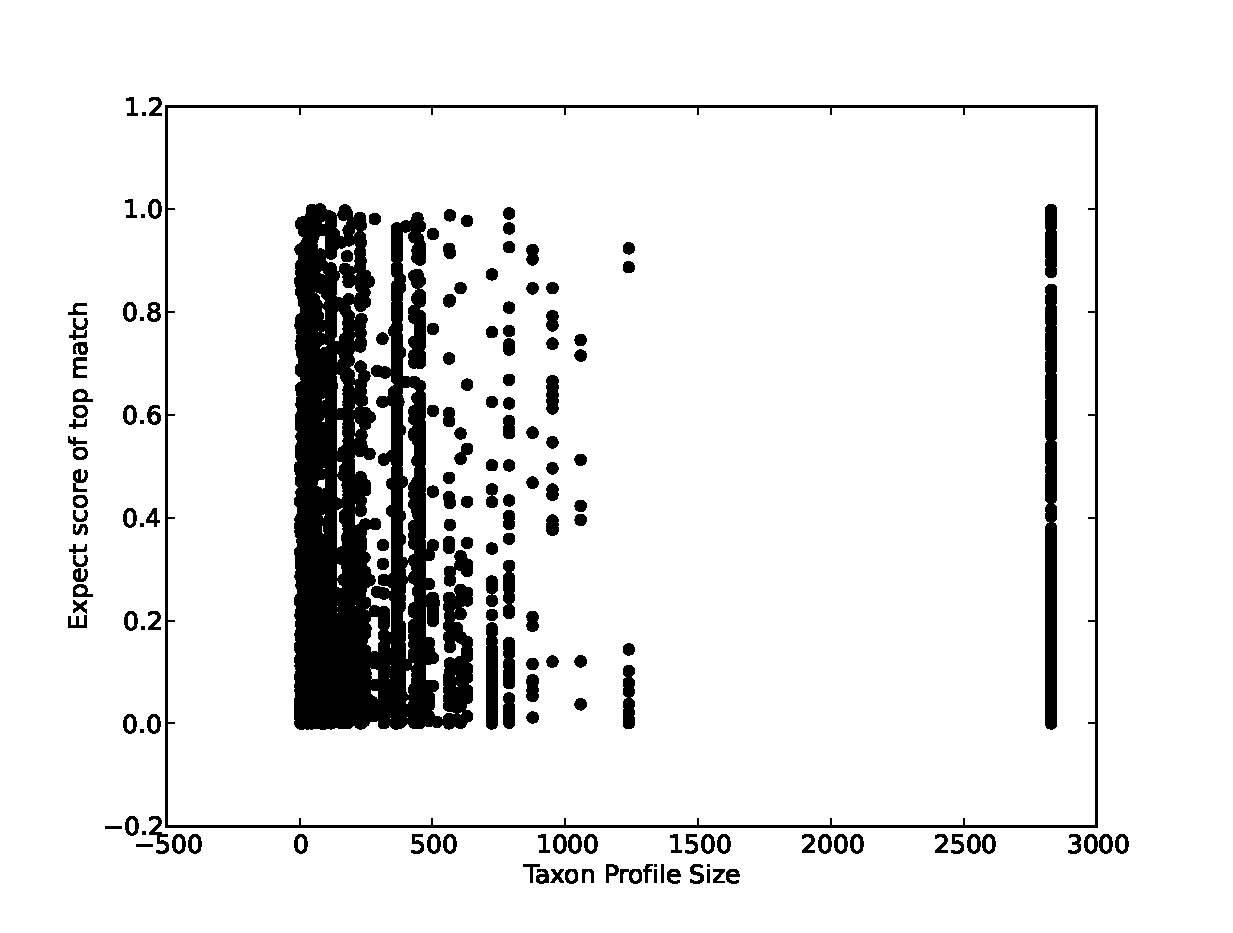
\includegraphics[width=1\textwidth]{TopMatches-ExpectDist.eps}
%\caption{\label{topmatchesdist} Distribution of the expect values of the top taxon matches for genes by size of the taxon's evolutionary profile.}
%\end{figure}

%%Semantic similarity result ranks from overall similarity and $E$ values were compared to estimate the difference in ranking between the two methods (Fig. \ref{ranks}). As expected, both rankings are strongly correlated; however, we do observe some differences.
%%
% \begin{figure}
% \centering
% 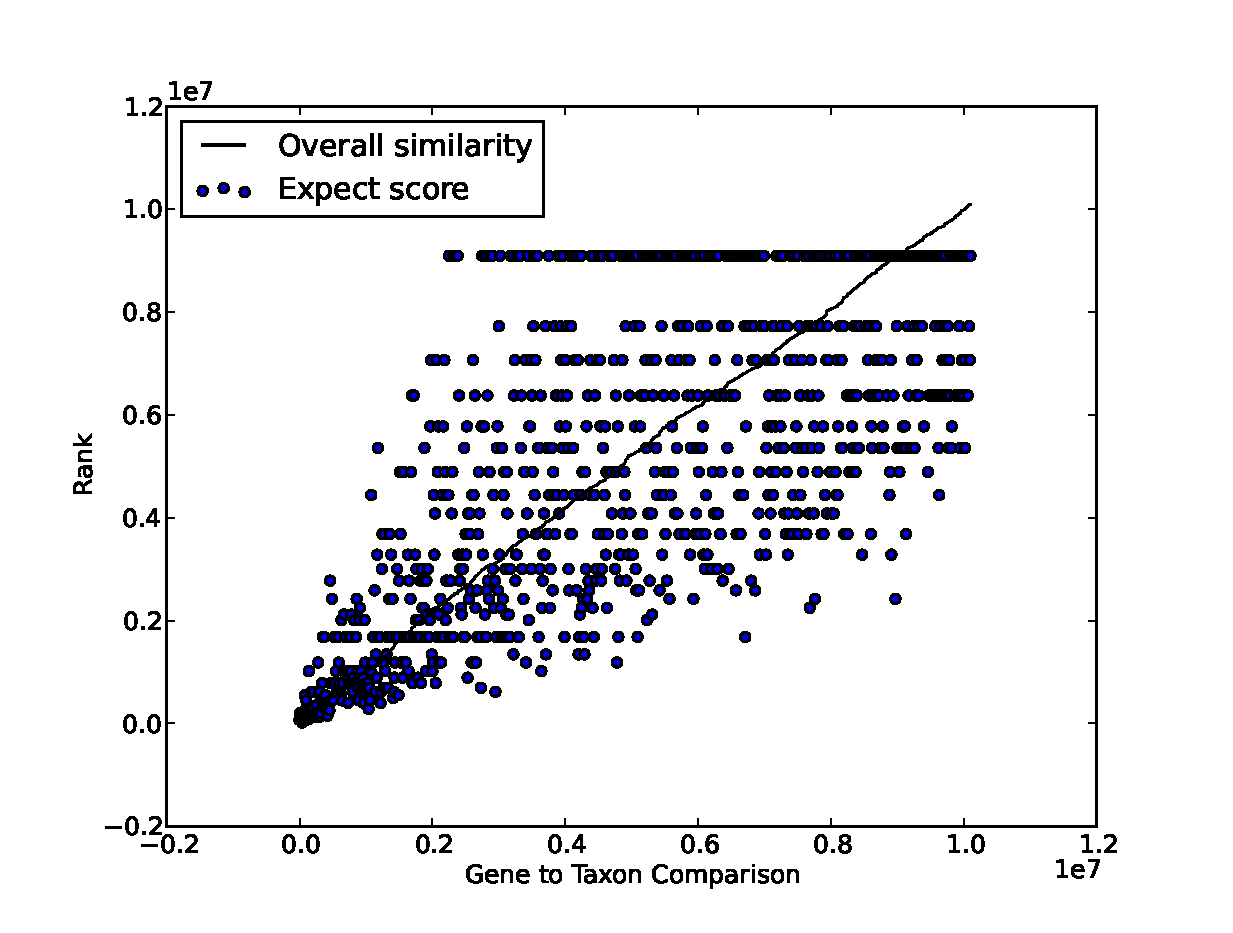
\includegraphics[width=1\textwidth]{RankComparisons.eps}
% \caption{\label{ranks} Comparison of overall similarity and Expect value ranks for semantic similarity searches.}
% \end{figure}

% 766 (approximately 10\%) of the 6,969 MICAs that contributed to semantic similarity scores were found to have IC differences greater than 0.25. The absolute value of the disparity was as high as 0.84 (Fig. \ref{disparityhistogram}).

% \begin{figure}
% \centering
% 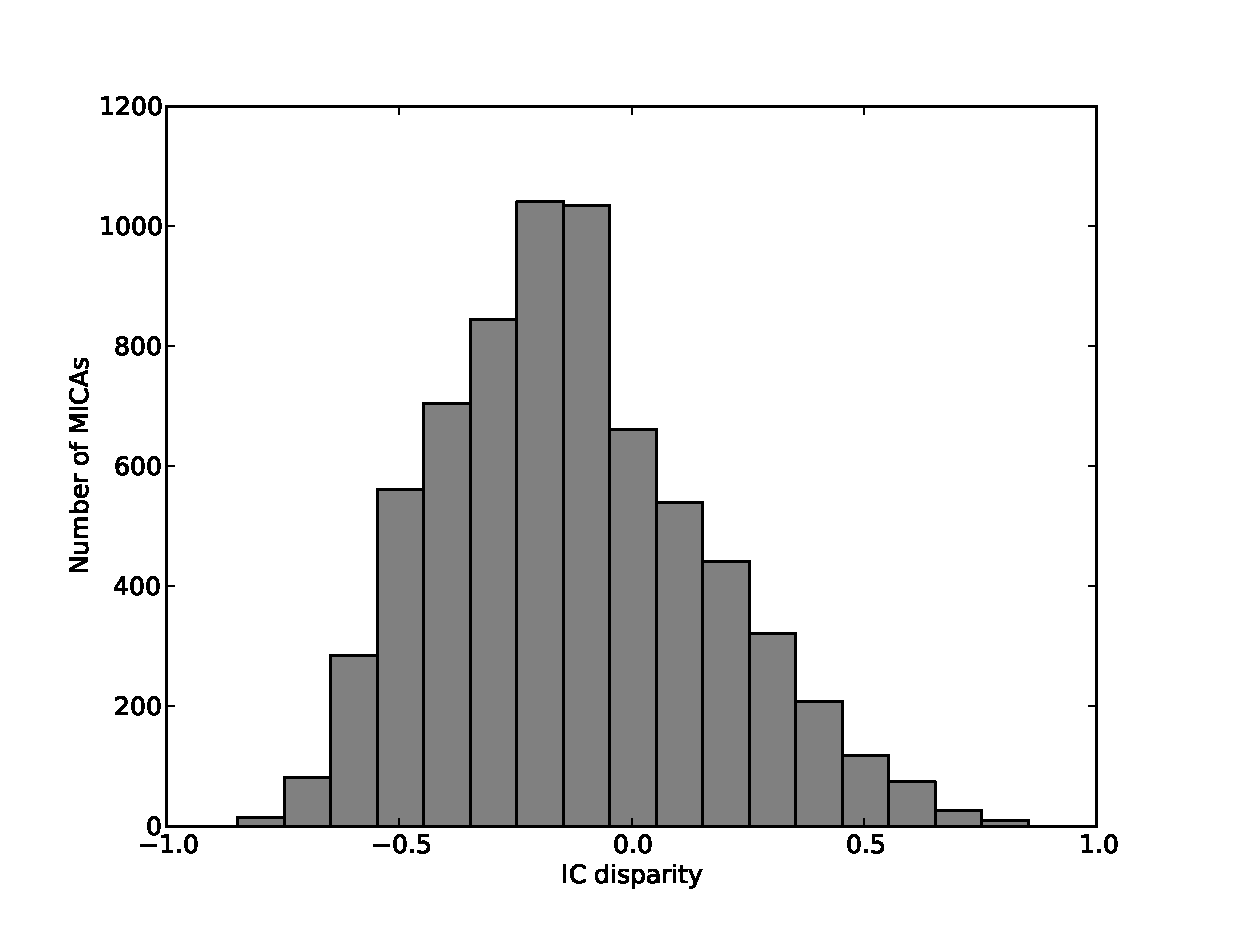
\includegraphics[width=1\textwidth]{Disparity-Histogram.eps}
% \caption{\label{disparityhistogram}Distribution of IC disparities for Most Informative Common Ancestors (MICAs) with unequal IC among gene and taxon profiles. N=6969.}
% \end{figure}
%%

\section{Discussion}

% So in the Discussion section, address one by one how well you've achieved each of the goals you've set for yourself in the Introduction, such as
% a comparison of the size of ontology you would need to reason over in the absence of the on-demand subsumer trickery
% how much reducing granularity from EQ to EA reduces the size of the ontology, and that it does not affect ranking of results
% how much inference of variation reduces the search space, and that the results returned are more biologically meaningful
% that the ranking of the top scores would be different (and biased) if 
% the distribution of E values to demonstrate that most match scores are not statistically significant (e.g. E approaching 1 or greater) but that a few are, and you have external evidence to suggest that these are real. 
% how useful are the E values?  Do the results reinforce that they are giving "correct" results?  (e.g. most matches are not statistically significant but the QQ plot and external evidence suggests that the top few are)
% how would the results be different/worse if we didn't use the Discrepancy Score? show that this matters.

In this study, we used an application in biology — connecting evolutionary variation among taxa to model organism genes based on similarity of phenotypes, to present the following: 1) models for reasoning over large combinations of multiple ontologies when pre-composed ontologies are not available, 2) approaches for data inference and search space reduction using domain knowledge when available data is sparse or missing, and 3) a framework to estimate statistical significance of semantic search matches from a database of ontological annotations. The methods presented here and the computational challenges we have addressed are common to other applications of semantic databases in the life sciences and beyond.

% how much does using inferred evolutionary profiles reduce the search space, and evaluate whether the results returned are more biologically meaningful. 

%%%% Not sure how to show that the results returned are more meaningful. 


More than 99\% of higher taxonomic nodes in VTO lack direct phenotype annotations indicating that computational inference is crucial for inferring evolutionary variation. Our inference algorithm inferred possible phenotypes for [X\%] of higher taxa, a substantial improvement from the 0.89\% with direct annotations. However, searching all of the X\% higher taxa is not meaningful since all of them might not indicate evolutionary variation. The inference algorithm reduced the search space by Y\% identifying the subset of taxa with evolutionary variation. Thus, the method was successful in addressing the missing data problem through inference and in reducing the search space thereby reducing computational complexity of the search.

% Compare the size of ontology you would need to reason over in the absence of the on-demand subsumer trickery
In the absence of a pre-composed EQ ontology, estimating similarity between evolutionary and gene phenotypes would require the infeasible task of reasoning over 36 million EQ classes - the combination of Uberon and PATO ontologies. Restricting the quality annotation granularity to the set of quality attributes significantly reduced the size of the combinatorial EQ space to 210,000 classes. The addition of corresponding EQ subsumers (built using OWL templates in \ref{reasoning}) and pre-composed gene phenotype classes brought the size of our comprehensive ontology to about 751,830 classes. This comprehensive ontology is still a significant reduction from the 36 million class space and enables reasoning over EQ annotations to estimate semantic similarity between gene and evolutionary phenotypes. 

% Is it an assumption (in which case can it be justified?) or is it a strategy (in which case is it successful?)
% It is a strategy based on the assumption that granularity of qualities doesn't matter. As a strategy, it is successful since it reduced the ontology size enough to do EQ similarity. However, we don't have results to show justify the assumption. 

In restricting the annotation granularity of quality annotations to high level attribute classes, we assume that the full level of quality annotation detail is not necessary for computing semantic similarity. One of the reasons for this assumption is that quality annotations are not as detailed as entity annotations which therefore might account for the majority of variation among annotations. The reduced quality reasoning paradigm infers potentially less informative common subsumers for annotation comparisons as compared to full quality reasoning. Thus, the gene to evolutionary profile similarities reported here are conservative lower-bound estimates that might be further enhanced if reasoning over the complete EQ hierarchy was feasible.
 
 
The initial linear regression model shows that taxon and gene profile size affect overall similarity indicating that results ranked by overall similarity would be biased by profile sizes. The difference in overall similarity and Expect value rankings indicates that Expect values "correct" the result ranking by accounting for profile size bias. A very small proportion of semantic similarity matches were found to have significant Expect values. The Q-Q plot and manual analysis of the top matches indicate that they are both statistically significant and biologically relevant.


% Does accounting for discrepancy matter?  How would the results be different/worse if we didn't use the Discrepancy Score?  Evaluate success. 

%%%% Results would not be any different if we didn't use the disparity scores. The disparity score doesn't change the results in any way. It just serves as a guide for users to interpret results. 

There are several challenges in inferring evolutionary variation and computing semantic similarity. We will discuss these challenges and identify areas for future work in subsequent paragraphs. 

Inference of evolutionary variation is currently guided by the vertebrate taxonomy ontology which is a poorly resolved form of the phylogenetic tree. The coarse resolution of the taxonomy might lead to the inference of evolutionary profiles that group evolutionarily independent phenotypes that might not have occurred at a single point in evolutionary history. Additionally, it is to be recognized that the ancestral reconstruction might assign evolutionary changes to incorrect taxa since it merely produces one of several potential parsimonious reconstructions of the taxonomy and not the right or unique reconstruction. These issues in the inference of evolutionary profiles have an effect on the biological relevance of the matched results. 

Information content based semantic similarity measures are sensitive to annotation biases specially if the data being compared comes from different domains (evolutionary phenotypes vs. gene phenotypes in our application). Certain sections of phenotypes might be extensively studied and annotated among model organism genes whereas the same phentoypes might be rarely observed in an evolutionary context. This would cause disparities in how informative a phenotype is perceived to be in different domains. Rarely studied and annotated phentoypes will be perceived to be more informative for the purposes of semantic similarity. Therefore, an informative annotation might be a result of actual biological rarity or simply an artifact of annotation bias. It is to be emphasized that our methods can only compute similarity as indicated by annotations (annotation similarity) and not actual biological similarity.

\section{Future Work}
Inferring evolutionary variation on a taxonomy with greater granular resolution will result in identification of evolutionary variation with better precision and therefore enable more meaningful biological matching to model organism gene phenotypes. A comparison of our similarity results from those using a better taxonomy would help to estimate the effect of taxonomy resolution on similarity searches. Additionally, we will explore other approaches of aggregating phenotypes for the inference of evolutionary variation. One of the major assumptions in restricting quality annotation granularity to high level attribute classes is that the loss of granularity on quality annotations does not affect similarity results substantially. We plan to conduct a comparison of similarity results from reasoning at the full quality level as opposed to the attribute level. This analysis will help to estimate the importance of quality annotations for estimating semantic similarity.Additionally, we will explore other OWL templates for creating relevant EQ subsumers. The size of the comprehensive ontology, the number of semantic searches, and profile sizes necessitate the pre-computation of all similarities before they can be queried on the KB. We plan to improve scalability and speed to enable on-the-fly semantic searches. 


\section{Availability}
The Phenoscape KB and semantic similarity search is available at http://kb.phenoscape.org. Source code is available under the MIT license from several repositories under the https://github.com/phenoscape organization, specifically phenoscape-owl-tools for the reasoning pipeline, including semantic similarity computation; phenoscape-kb-services for data services; and phenoscape-kb-ui for the web user interface.  \textbf{(Needs to be updated)} The code and a dataset representing a freeze of the semantic similarity search results reported here is available from Zenodo (reasoning pipeline: http://dx.doi.org/10.5281/zenodo.17247; web services: http://dx.doi.org/10.5281/zenodo.17248; web user interface: http://dx.doi.org/10.5281/zenodo.17249).

\section{Acknowledgments}
The Phenoscape project is funded by NSF grants DBI-1062404 and DBI-1062542, and supported by the National Evolutionary Synthesis Center (NESCent), NSF EF-0905606. 

\begin{table}
\caption{A glossary of variables used in the study.}
    \centering
    \begin{tabularx}{1\textwidth}{XX}
        \hline
 $A$ & An annotation in a gene phenotypic profile or an evolutionary profile. \\
 $\alpha$ & Evolutionary profile size co-efficient in the linear regression. \\
 $\beta$ & Gene phenotypic profile size co-efficient in the linear regression. \\
$C$ & Comprehensive ontology for semantic similarity reasoning \\
  $i$ & Intercept from the multiple linear regression. \\
$D$ & Difference between the IC of the MICA among evolutionary profiles and gene phenotypic profiles. \\
$E$ & Entity class \\
 $f(N)$ & Number of taxa annotated directly to $N_i$ or to any node subsumed by $N_i$.  \\
 $IC$ & Information Content of a $MICA$. \\
 $IC_T$ & $IC$ of a MICA among evolutionary profiles. \\
 $IC_G$ & IC of a MICA among gene phenotypic profiles. \\
 $IC_{max}$ & Maximum IC score possible for a particular dataset. \\
 MICA & Most informative common ancestor of a pair of annotations; one from a gene phenotypic profile and another from an evolutionary profile. \\
 $nIC$ & Normalized IC computed from $IC$ to fit the range [0,1]. \\
$N$ & A node in an ontology. \\
$Q_A$ & Attribute quality class from PATO. \\ 
 $R_R$ & Raw residuals from the linear regression. \\
 $R_S$ & Studentized residuals from the linear regression. \\
 $S_A$ & similarity between a pair of annotations; one from a gene phenotypic profile and another from an evolutionary profile. \\
 $S_O$ & overall similarity between a gene phenotypic profile and a taxon's evolutionary profile.  \\
  $S_O'$ & overall similarity as predicted by a multiple linear regression with gene phenotypic profile size, evolutionary profile size as the independent variable and overall similarity as the independent variable. \\
 $\sigma$ & Estimate of standard deviation of the residuals. \\
 
 $T$ & Number of taxa with evolutionary profiles. \\
 $X$ & Size of a given taxon's evolutionary profile. \\
 $Y$ & Size of a given gene phenotypic profile. \\
 
 \end{tabularx}
\end{table}


       
\bibliographystyle{abbrv}
\bibliography{Postdoc-References}  % sigproc.bib is the name of the 
\end{document}
